%Notes on Infinite Sets from How to Prove It by Daniel J. Velleman
\documentclass{article}
\usepackage{amsmath} 
\usepackage{amsfonts}
\usepackage{amssymb}
\usepackage{indentfirst}
\usepackage{graphicx}
\graphicspath{ {c:/Users/Polymathykhan/Documents/GitHub/polymathykhan.github.io/images/} }

\begin{document}
\setlength\parindent{24pt}
\begin{center}
\begin{huge}
Notes on Infinite Sets
\end{huge}
\\from Velleman's How to Prove It: A Structured Approach
\newline by Ibraheem Khan
\end{center}

\section{Equinumerous Sets}

\par Suppose A and B are sets. We'll say that A is equinumerous with B if there is a function f: A $\to$ B that is one-to-one and onto, that is, it is a bijection. Let A $\sim$ B denote that A is equinumerous to B. A set A is finite if there exists some n $\in$ $\mathbb{N}$ such that $\{$i $\in \mathbb{Z}^{+}$ $|$ i $\leq$ n$\}$ $\sim$ A. Essentially, if there is some sequence of or some selection of positive integers that are less than n and we collect these numbers into a set and also if this set is equinumerous to our set A, then set A is finite. Otherwise, A is an infinite set. Its cardinality, however, is not to be conflated with this notion of infinity. Finite cardinalities simply refers to the number i in finite sets as it is merely the number of elements in a set. However, in infinite sets cardinalities must be found via investigation of such bijections. Further, it is known that $\sim$ is an equivalence relation as it is reflexive, symmetric, and transitive. Refer to the notes done in class from Book of Proof for other trivialities, (such as finding particular one to one correspondences). 
\\
\par We now expand our notion of countable sets as being denumerable sets- that is sets A $\sim$ $\mathbb{Z}^{+}$ or those that are finite. Uncountable sets will be defined as those that are not countable. Uncountable sets are not necessarily sets whose cardinalities are equivalent to $\mathbb{R}$. 
\\
\par Here are some interesting equivalent statements:

\begin{enumerate}
\item A is countable.
\item Either A = $\varnothing$ or there is a function f: $\mathbb{Z}^{+} \to$ A that is surjective.
\item There is a function f: A $\to \mathbb{Z}^{+}$ that is bijective.
\end{enumerate}
\textbf{Theorem 1}
\textit{Statements 1, 2, and 3 are logically equivalent}
\begin{flushleft}
1 $\implies$ 2
\end{flushleft}
\par A is a countable set. Thus, either A is denumerable or finite. Suppose A is denumerable. Then, by definition, there is a bijection f: $\mathbb{Z}^{+} \to$ A. Now, suppose A is finite. Thus, its cardinality is either $\varnothing$ or some number n as defined above. If $|$A$|$ = $\varnothing$ then clearly the first conditional in the OR proposition is true. If it is not, then $|$A$|$ = n. We want to prove that there exists some surjective function from the positive integers to A given that $|$A$|$ = n. Intuitively, we want to map all elements of the positive integers to all elements of A. This can be done by constructing the following set $\mathcal{G}$: $\{$i $\in \mathbb{Z}^{+}$ $|$ i $\leq$ n$\}$. Now, let $\mathcal{G} \to$ A be a bijection, g, given n is the number of elements of A. To clarify this construction see the above definition of finite. Let a $\in$ A. Now, we define $f$: $\mathbb{Z}^{+} \to$ A :
\[ f(i) =
	\begin{cases} 
      g(i) & \text{if } i \leq n \\
      a_{0} & \text{if } i > n \\
   \end{cases}
\]
\par Clearly, this function is surjective as all A is mapped. The function $g$ simply assigns positive integers to our set. For example, one such assignment, or mapping, would be $\{$1,2,3,4,5$\}$ to a set A=$\{$Apple, 5, Photon, $\prod_{i=1}^{\infty} \zeta_{i}$, Reader$\}$. Clearly, the set A is a rather exotic set but $\mathcal{G}$ simplifies the set down to ordered, positive integers via the function $g^{-1}$. We know the inverse exists as we know g is a bijection.
\\
\\
\begin{flushleft}
2 $\implies$ 3
\end{flushleft}
\par If A is the null set, then the empty set itself is the bijection from A to $\mathbb{Z}^{+}$. To explore the intricacies of this we will explore the various subtleties of empty sets and empty functions. \textbf{Empty sets} are the \textit{unique} sets having no elements with cardinality zero. Many statements regarding sets and other mathematical objects \textit{vacuously} hold true. Empty sets hold the following properties $\forall$ sets $A$:
\begin{enumerate}
\item $\varnothing \subseteq A$
\item $A \subseteq \varnothing \implies A=\varnothing$
\item $A \cup \varnothing = A$
\item $A \cap \varnothing = \varnothing$
\item $A \times \varnothing = \varnothing$
\item $\mathcal{P}$($\varnothing$) $= 2^\varnothing = \{\varnothing\}$ (that is, the set containing the null set)
\end{enumerate}
\par We will not consider the various set theory and ontological ideas surrounding the notion of the empty set and nothingness in general. Instead, we shall, for now, push on to describe the empty function from the definition of a function itself:
\[
\forall z (z\in F\implies\exists x\exists y(z=\{\{x\},\{x,y\}\})\land\\  \forall x(\exists z\exists y(z\in F\land z=\{\{x\},\{x,y\}\})\implies \\ 
\]
\[
(\forall u\forall v(\exists z\exists w((z\in F\land w\in F\land z= \{\{x\},\{x,v\}\}\land w=\{\{x\},\{x,u\}\})\implies u=v)
\]
\par I will give credits to Asaf Karagila on StackExchange for this definition. The key to understanding this lies in understanding the logical bounded quantification of statements as $\forall x\in A(P(x))$ which really should be read as $\forall x(x\in A\implies P(x))$. One must recall the truth table of implications which show that the statement is only false when the condition is true but the resolution is false. So to provide an explication of our above definition of a function, it states that we have some condition. This condition is true only when two subconditions are true given the logical AND conjunction. The first subcondition states that for all elements $z$ that are in the function $F$. Now note the following: 
\[
{F\text{: } D \to C} \implies F \subseteq D \times C
\]
\par Thus, we can see that functions are in fact binary relations, that is a collection of ordered pairs, such that it is a subset of the cartesian product of the domain and codomain. Since functions are in fact binary relations they are also sets, specifically, a set having all its elements be ordered pairs. According to Kuratowski, ordered pairs are defined as
\[
(x,y) = \{\{x\}, \{x,y\}\}
\]
Thus, $z$ is an element of $F$ and since it is an element of $F$ it is an ordered pair. Now, for all such $z$, if $z$ is an element of $F$, then it is implied that there exists some $x$ and $y$ such that the definition of an ordered pair is satisfied for $z$. The second subcondition states that for all $x$ there must exist $z$ and $y$ such that the ordered pair is formed. In effect, the condition essentially states that we have a function composed of elements $z$, that $z$ is defined as such, and that we have fixed our elements $x$, or really our left-coordinate.
\par The implication then leads us to show that given this information, for every right-coordinate $x$, there will only be \textit{one} such corresponding $y$ or right-coordinate in the only possible ordered pair for that $x$. That is, if we have two right-coordinates $u$ and $v$ and we have ordered pairs $(x,u)$ and $(x,v)$ then $u=v$. This agree with out intuitive definition of a function in that if we some $\mathbf{X}$ $\in$ $\mathcal{D}$($F$) then there is a unique $\mathbf{Y}$ $\in$ $\mathcal{C}$($F$) such that $\mathbf{X}$$F$$\mathbf{Y}$ or really that ($\mathbf{X}$,$\mathbf{Y}$) $\in F$. Now, the empty function is a function much in the same way that the empty set is a set of real numbers or elephants. The set contains no elements so it may vacuously hold true for any restriction including the definition of functions as 
\begin{itemize}
\item The empty set is a collection of ordered pairs
\item The empty set has no ordered pairs
\item $x$ is the fixed left coordinate of these non-existent ordered pairs
\item The condition then vacuously holds true
\item No left-coordinate has no two or more equal right-coordinates in $\varnothing$ as $\varnothing$ has no $(x,y)$
\item The implication holds true, thus $\varnothing$ is a function.
\end{itemize}
\par Thus, the empty set is indeed a function- in particular it is the \textit{unique} empty function for some set S where
\[
\varnothing: \varnothing \to S \text{ as } \varnothing \times S = \varnothing
\]
\par Now, it is important to note that this function is always surjective. This is easy to see as any function from $\varnothing$ to some set $A$ has to be a subset of the Cartesian product between the two, but the cartesian product of $\varnothing$ with $A$ is equal to the function $\varnothing$. Thus, $\varnothing$ is always a surjection. To clarify, I will be referring to $\varnothing$ as any particular function that is a member of the class of functions $f$: $\varnothing \to A$ \text{} $\forall A$. Injectivity vacuously holds as well due to the fact that if given $f(x)=f(y)$ $\implies$ $x=y$ as no such $(x,y)$ exist for the empty function. Thus, $\varnothing$ is always a bijection. 
\par Now, with that excursion out of the way we may continue on with the proof that 2 implies 3. Now, we suppose $g$: $\mathbb{Z}^{+} \to A$ is a surjection. Then an injection $I$: $A \to \mathbb{Z}^{+}$ necessarily exists by the well-ordering-principle (least integer principle) as for any instance where $g(n)=a$ we may select the smallest $n$ and define $I(a) =$ the smallest $n$ for which $g(n)=a$. Further, $g \circ I = i_{a}$ that is $g$ composed with $I$ is the identity map on set $A$. This too implies that $I$ is one-to-one.  
\begin{flushleft}
3 $\implies$ 1
\end{flushleft}
\par We now show that if there is an injection from some set to the positive integers (or natural numbers) then the set is countable- that is, it is denumerable or it is finite. Now, since $I$ is one-to-one $\mathcal{D}$($I$) $\sim \mathcal{C}$($I$). Further, $\mathcal{D}$($I$) $= A$ and $\mathcal{C}$($I$) $\subseteq \mathbb{Z}^{+}$. Thus, since the set of positive integers is countable, a subset of it is countable, and so since the domain of our function has the same cardinality as this subset of the positive integers that is the codomain of our function it too must be countable. And so, our proof of the given theorem is complete.
{$\blacksquare$}
\section{Properties of Infinite Sets and Cantor's Theorem}
\par We will now prove that: $A \times B$ and $A \cup B$ are both countable if both $A$ and $B$ are countable. Obviously, if either $A$ or $B$ is uncountable then their Cartesian products and unions are also uncountable. Since $A$ and $B$ are both countable there exists functions $f$:$A \to \mathbb{Z}^{+}$ and $g$:$B \to \mathbb{Z}^{+}$. Now, clearly, if the sets are finite their product is finite but if they are denumerable there is more to be said, that is why we imply the denumerability of our sets as we can then assert that the functions $f$ and $g$ are one-to-one and onto. Thus, to prove that $A \times B$ is countable we simply show that $\mathbb{Z}^{+} \times \mathbb{Z}^{+}$ is denumerable as we can define a function $h$:$A \times B \to \mathbb{Z}^{+} \times \mathbb{Z}^{+}$. We know this function is one-to-one if defined as follows: 
\[
h(a,b)=(f(a),g(b))
\]
\par It is easy to show that is a surjection as $f$ and $g$ assure all of $\mathbb{Z}^{+}$ and any combination of $(a,b)$ may be chosen. Injectivity can also be easily shown as $f$ and $g$ are also both injective. Thus we must show that $\mathbb{Z}^{+} \times \mathbb{Z}^{+}$ is countable.
\\
\\
\textbf{Theorem 2}
\textit{$\mathbb{Z}^{+} \times \mathbb{Z}^{+}$ is countable}
\par To show that $\mathbb{Z}^{+} \times \mathbb{Z}^{+}$ is countable we will use the Cantor-Pairing function which is defined as
\[
\pi: \mathbb{Z}^{+} \times \mathbb{Z}^{+} \to \mathbb{Z}^{+}
\]
\[
\pi(a,b)=\frac{1}{2}(a+b)(a+b+1)+b
\]
\par To prove that this is a bijection, we may simply find the inverse of this function.
Let $\pi(x,y)=z=t+y$ where $w=x+y$ and $t$ is the triangle number of $w$- that is $t=\frac{1}{2}w(w+1)$. Thus, we must solve for $x$ and $y$ from $z$. Note that $x$ and $y$ are natural numbers, thus, so must be $w$ as well as $t$ and hence $z$. Now, note $w^2+w=2t$ so if we solve the quadratic equation
\[
w^2+w-2t=0
\]
We find that 
\[
w=\frac{\sqrt{8t+1}-1}{2}
\] 
This function is strictly increasing. We then show the follow inequalities:
\[
t \leq z=t+y
\]
\[
t+w+1=t+x+y+1=(t+y)+x+1 > z
\]
\[
t+(w+1)=\frac{(w+1)^2+(w+1)}{2}
\]
Thus, we may note that 
\[
w \leq \frac{\sqrt{8z+1}-1}{2}
\]
We will now prove that 
\[
w \leq \frac{\sqrt{8z+1}-1}{2} < w+1=\frac{(\frac{\sqrt{8t+1}-1}{2}+1)^2+(\frac{\sqrt{8t+1}-1}{2}+1)}{2}
\]
Expanding we get
\[
-2\sqrt{8t+1}\sqrt{8t+8y+1}+16t+8y+2 < 2t+\frac{3}{2}
\]
Note
\[
\sqrt{8t+8y+1}>\sqrt{8t+1}
\]
Thus, we may replace the $\sqrt{8t+1}$ term with $\sqrt{8t+8y+1}$ to prove the inequality. In doing so we find:
\[
-8y<2t+\frac{3}{2}
\]
Which is clearly true. Thus,
\[
w=\left \lfloor{\frac{\sqrt{8z+1}-1}{2}}\right \rfloor
\]
We may now solve for $x$ and $y$ in terms of $z$:
\[
x=\left \lfloor{\frac{\sqrt{8z+1}-1}{2}}\right \rfloor - z + \frac{(\left \lfloor{\frac{\sqrt{8z+1}-1}{2}}\right \rfloor)^2+(\left \lfloor{\frac{\sqrt{8z+1}-1}{2}}\right \rfloor)}{2}
\]
\[
y=z - \frac{(\left \lfloor{\frac{\sqrt{8z+1}-1}{2}}\right \rfloor)^2+(\left \lfloor{\frac{\sqrt{8z+1}-1}{2}}\right \rfloor)}{2}
\]
Thus the Cantor-Pairing function is invertible and therefore it is a bijection. This implies that the cartesian product of $\mathbb{Z}^{+}$, which is also denoted, $\mathbb{N}$, with itself is countable.
{$\blacksquare$}
\par Due to the above theorem the property that the cardinality of the cartesian products of countable sets is countable has been proven. As a result, the Cantor-Pairing Function may be generalized with similar properties (one may also prove these properties via induction):
\[
\pi ^{{(n)}}:{\mathbb  {N}}^{n}\to {\mathbb  {N}}
\]
\[
\pi ^{{(n)}}(k_{1},\ldots ,k_{{n-1}},k_{n}):=\pi (\pi ^{{(n-1)}}(k_{1},\ldots ,k_{{n-1}}),k_{n})\,.
\]
\par We now prove that the union of countable sets is also countable. We first consider a function $h$: $A \cup B \to \mathbb{Z}$ defined as follows:
\[h(x) =
	\begin{cases} 
      f(x) & \text{if } x \in A \\
      -g(x) & \text{if } x \not\in A \\
   \end{cases}
\]
\par While this function is clearly not a surjection (as it fails to map 0) it is obviously injective. Now, we simply let $j$: $\mathbb{Z} \to \mathbb{N}$ be a one-to-one, onto function and my the preservation of injectivity in compositions we find $j \circ h$: $A \cup B \to \mathbb{N}$ is one-to-one. Thus, it must be countable. Bijectivity is not necessary (but is of course sufficient) to prove countability, refer to Theorem 1. We will now prove an interesting variant of this idea- that the union of countably many countable sets is countable. An intuition to this idea might be thinking of even and odd numbers. The set of evens is infinitely countable as is the set of odds. However, instead of breaking up the naturals into evens and odds one could break them up into countably many ``even" and ``odd" subsets. Consider the following progression:
\[
1\:2\:3\:4\:5\:6\:7\:8\:9\:10\:11\:12\:13\:14\:15\:16\:17\:18\:19\:20\:21\:22\:23\:24\:25\:26\:27\:28\:29\:30...
\]
\[
1\:3\:5\:7\:9\:11\:13\:15\:17\:19\:21\:23\:25\:27\:29...
\]
\[
1\:5\:9\:13\:17\:21\:25\:29...
\]
\[
1\:9\:17\:25...
\]
\[
1\:17...
\]
\[
.
.
.
\]
\par This one may think of being as an ``odd-only" progression. Essentially, I have created a subset of the natural numbers by selecting ``every other element starting from the first element in the set" or really by selecting the ``odd" members of the set. However, at each step in the process I had the choice of choosing the ``odd" members or the ``even" members. For example, at the second to last step I could have constructed as follows:
\[
1\:9\:17\:25...
\]
\[
9\:25...
\]
\[
.
.
.
\]
\par This would have led to a different subset even if I continued with the policy of only choosing ``odd" members. Thus, we may construct infinitely many subsets of the natural numbers that in turn have infinitely many elements as we have infinite choices as we have infinitely many steps in this construction and two choices at each step: to select the ``odd" or ``even" members for the next step-set. Thus, one could think that ``after" this infinite process we should have infinitely many subsets of the natural numbers that have infinitely many elements. However, since these are all subsets of the natural numbers, then, should we label each ``final" subset $S$, then we should expect:
\[
\bigcup_{n=1}^{\infty} S_{n}=\mathbb{N}
\]
\par Considering the union of these sets having infinitely many elements is equivalent to a countable set it would lead us to believe that these sets by themselves should also be countable. As such, this would provide us the much necessary intuition to proceed with the proof that the union of countably many countable sets is indeed countable. Note, that we have countably many infinite choices as well (we procured each ``choice" via a procedural list and as we shall see list if we can sequence objects then the set of those objects is countable. Further one may conceive of this as a choice-tree and labeling nodes on such a graph is a trivial task, this labeling is in effect forming a sequence). One final formality to consider in this intuition is the notion of these sets being disjoint.``After" the process all the sets produced will be disjoint so their intersections will be the null set. However, the property we aim to prove does not require that the countably many sets in question be disjoint.
\par Consider some family of sets (note a family may be contained in a set but is not a set in and of itself), $\mathcal{F}$ that is countable and that every element is $\mathcal{F}$ is also countable. Then $\cup \mathcal{F}$ is also countable. Suppose $\mathcal{F} = \varnothing$ then clearly
\section{The Cantor-Schr\"oder-Bernstein Theorem}
Stuff will go here about that...
\section{Appendix-Deriving the Cantor Pairing Function}
\par Pairing functions are any bijective function that maps (computably so) $\mathbb{N} \times \mathbb{N}$ to $\mathbb{N}$. We will now proceed to derive this function from the familiar diagonal argument: 
\begin{figure}[h]
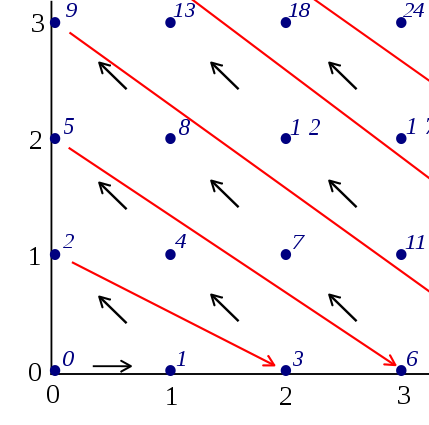
\includegraphics[width=4cm]{CantorPF}
\centering
\end{figure}
\par Above is a visual of how the function should map each coordinate pair to a natural. It is important to note that this kind of diagonal progression is standard across set theory and even in some areas of computer science. For example, a similar trick is used to count the rationals (the "next" idiom does not work on the rationals as a way to count as there is no computable (in finite time) rational directly adjacent to some rational $n$): 
\begin{figure}[h]
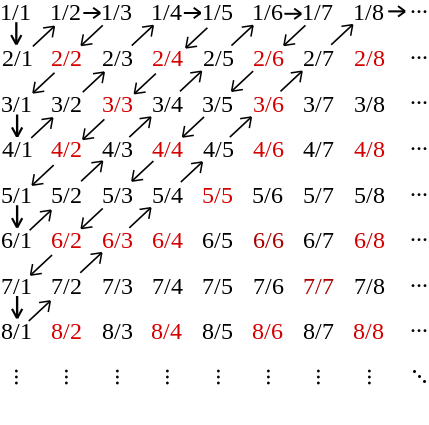
\includegraphics[width=4cm]{CountingRationals}
\centering
\end{figure}
\par Now all that is left is to translate the graphical interpretation of our function into algebra. Now one can easily confirm from the above image (which defines our function) that:
\[
\pi (x,y)+1=\pi (x-1,y+1)
\]
\par Then, we must find suitable boundary conditions for our function. Essentially, we want to use the above definition with some boundary conditions to find a polynomial in the real euclidean plane. Should the proof be done procedurally one would have first tested a first-order polynomial (however clearly this will not work) so we will first attempt to construct a second order polynomial that fits our criteria. 
\par Now of course, we know that $\pi(0,0)=0$. This will be the initial step. Further, may consider the function along the x and y axes. Along them we have the following description:
\[
\pi (0,k)+1=\pi (k+1,0)
\]
We now consider a general 2-variate 2nd order polynomial:
\[
\pi (x,y)=ax^{2}+by^{2}+cxy+dx+ey+f
\]
From our initial step it is obvious that $f=0$. We will now apply our boundary conditions to find:
\[
bk^{2}+ek+1=a(k+1)^{2}+d(k+1)
\]
Now, remember that this $k$ applies to all naturals and is not a variable in this context. The statement is true for all naturals k. Thus, if we simply let $k=0$ we find $d=1-a$. Following some algebra we arrive at
\[
k^2(b-a)+k(e-a-1)=0
\] 
Thus, $b=a$ and $e=1+a$. Should we add this newly found information using our first definition we arrive at (by writing everything in terms of a and c):
\[
{\begin{aligned}\pi (x,y)+1&=a(x^{2}+y^{2})+cxy+(1-a)x+(1+a)y+1\\&=a((x-1)^{2}+(y+1)^{2})+c(x-1)(y+1)+(1-a)(x-1)+(1+a)(y+1)\end{aligned}}
\]
Following much algebra we find
\[
(2a-c)(x-y)=4a-2
\]
\par We know that at $(0,0)$ there is a natural number mapped by $\pi$. Thus, if we let $x=0$ and $y=0$ then we see that $a=\frac{1}{2}$. Substituting that back into the expression we find $c=1$. Solving for the rest we find $e=\frac{3}{2}$ and that $d=1-a=\frac{1}{2}$ and of course $f=0$. Thus, we may now add this back into the final equation:
\[
{\begin{aligned}\pi (x,y)&={\frac {1}{2}}(x^{2}+y^{2})+xy+{\frac {1}{2}}x+{\frac {3}{2}}y\\&={\frac {1}{2}}(x+y)(x+y+1)+y,\end{aligned}}
\]
And thus we have derived the Cantor-Pairing Function.

\end{document}

